%%%%%%%%%%%%%%%%%%%%%%%%%%%%%%%%%%%%%%%%%%%%%%%%%%%%%%%%%%%%%%%%%%%%%%%%%%%%%%%
\section{Test Case 2}
\label{sec:test-case2}
%%%%%%%%%%%%%%%%%%%%%%%%%%%%%%%%%%%%%%%%%%%%%%%%%%%%%%%%%%%%%%%%%%%%%%%%%%%%%%%

The second test case was designed to investigate the impact of the groupwise reaction rate errors in the context of an eigenvalue calculation for a PWR benchmark. The influence of the energy-integrated reaction rate errors on the global eigenvalue is evaluated in~\autoref{sec:case2-eigenvalue-bias}, while ~\autoref{sec:case2-flux-bias} quantifies the relationship between the bias and reaction rate errors in the energy groups with large resonant capture cross sections.

%%%%%%%%%%%%%%%%%%%%%%%%%%%%%%%%%%%%%%%%%%%%%%%%%%%%%%%%%%%%%%%%%%%%%%%%%%%%%%%
\subsection{Eigenvalue Bias}
\label{sec:case2-eigenvalue-bias}

The OpenMC Monte Carlo code was used to tally MGXS in seventy energy groups and to compute a reference eigenvalue for the second test case benchmark. Reference eigenvalues are presented in~\autoref{tab:keff-reference} for simulations with ``normal'' anisotropic scattering, and for the case when OpenMC's ``iso-in-lab'' feature was employed. The two reference OpenMC simulations were also used to tally separate MGXS libraries to quantify the isotropic in lab scattering approximation used in OpenMOC and to isolate it from the flux separabilty approximation.

\begin{table}[h!]
  \centering
  \caption{Reference OpenMC eigenvalues for a 2D fuel pin.}
  \label{tab:keff-reference} 
  \begin{tabular}{c c}
  \toprule
  {\bf Anisotropic} &
  {\bf Isotropic in Lab} \\
  \midrule
  1.17488 $\pm$ 0.00001 & 1.17422 $\pm$ 0.00001 \\
  \bottomrule
\end{tabular}
\end{table}

The MGXS were employed by a series deterministic multi-group transport simulations to quantify the interaction between the energy and spatial approximations. The effects of energy discretization was analyzed by collapsing the 70-group MGXS library to coarser group structures used by the CASMO code. The MOC Flat Source Region (FSR) spatial discretization meshes were varied with constant-by material MGXS in each FSR to quantify the interaction between the energy and spatial approximations. In particular, 1, 4 or 16 radial rings were used to discretize both the fuel and moderator, while 8 azimuthal sectors were used to discretize the fuel, gap, clad and moderator. The MGXS were computed using tally meshes in OpenMC identical to the FSR meshes used by OpenMOC. All OpenMOC simulations used 128 azimuthal angles and 0.01 cm track spacing for the characteristic track laydown.

%The results underline the complex interactions between discretizations in energy and space which are impacted by the loss of angular information due ot the flux separability approximation. 

In the results that follow, the bias $\Delta\rho$ compares the eigenvalue $k_{eff}^{MOC}$ computed by OpenMOC to that of the reference eigenvalue $k_{eff}^{MC}$ computed by OpenMC in units of pcm:

\begin{equation}
\label{eqn:delta-rho}
\Delta\rho = \left(k_{eff}^{MOC} - k_{eff}^{MC}\right) \times 10^{5}
\end{equation}

\noindent The eigenvalue bias for the ``normal'' anisotropic and ``iso-in-lab'' simulations are presented in~\autoref{tab:keff-bias-aniso} and~\autoref{tab:keff-bias-iso-in-lab}, respectively, for varying energy group structures and FSR spatial discretizations. The results illustrate a strong interaction between the energy and spatial meshes used to solve the multi-group transport equation.

%In particular, the eigenvalue bias grows in magnitude with more energy groups and FSRs but is largely insensitive to the the elimination of the isotropic scattering approximation.

\begin{table}[h!]
  \centering
  \caption{The eigenvalue bias with anisotropic scattering.}
  \label{tab:keff-bias-aniso} 
  \begin{tabular}{c S[table-format=6.1] S[table-format=6.1] S[table-format=6.1]}
  \toprule
  & \multicolumn{3}{c}{{\bf FSR Discretization}} \\
  \midrule
  \multicolumn{1}{c}{{\bf \# Groups}} &
  {\bf 1$\times$} & {\bf 4$\times$} & {\bf 16$\times$} \\
  \midrule
1 & 67 & 63 & 92 \\
2 & 22 & -56 & -51 \\
4 & -58 & -128 & -135 \\
8 & -75 & -182 & -197 \\
16 & -73 & -190 & -207 \\
25 & -128 & -246 & -268 \\
40 & -131 & -261 & -288 \\
70 & -132 & -267 & -297 \\
  \bottomrule
\end{tabular}
\end{table}

%\begin{table}[h!]
%  \centering
%  \caption{The eigenvalue bias with transport-corrected MGXS.}
%  \label{tab:keff-bias-aniso} 
%  \begin{tabular}{c S[table-format=6.1] S[table-format=6.1] S[table-format=6.1]}
%  \toprule
%  & \multicolumn{3}{c}{{\bf FSR Discretization}} \\
%  \midrule
%  \multicolumn{1}{c}{{\bf \# Groups}} &
%  {\bf 1$\times$} & {\bf 4$\times$} & {\bf 16$\times$} \\
%  \midrule
%1 & 53 & 75 & 72 \\
%2 & 37 & 1 & 4 \\
%4 & -58 & -92 & -109 \\
%8 & -74 & -145 & -170 \\
%16 & -67 & -154 & -183 \\
%25 & -124 & -221 & -245 \\
%40 & -130 & -238 & -265 \\
%70 & -131 & -281 & -274 \\
%  \bottomrule
%\end{tabular}
%\end{table}

\begin{table}[h!]
  \centering
  \caption{The eigenvalue bias with isotropic-in-lab scattering.}
  \label{tab:keff-bias-iso-in-lab} 
  \begin{tabular}{c S[table-format=6.1] S[table-format=6.1] S[table-format=6.1]}
  \toprule
  & \multicolumn{3}{c}{{\bf FSR Discretization}} \\
  \midrule
  \multicolumn{1}{c}{{\bf \# Groups}} &
  {\bf 1$\times$} & {\bf 4$\times$} & {\bf 16$\times$} \\
  \midrule
1 & 80 & 55 & 66 \\
2 & 141 & 29 & 34 \\
4 & 27 & -43 & -57 \\
8 & 26 & -85 & -102 \\
16 & 35 & -91 & -111 \\
25 & -31 & -158 & -182 \\
40 & -38 & -174 & -202 \\
70 & -39 & -182 & -211 \\
  \bottomrule
\end{tabular}
\end{table}

In particular, the eigenvalue bias varies by up to 350 pcm between energy group structures and nearly 200 pcm between FSR discretizations. The use of isotropic in lab scattering in OpenMC reduces the magnitude of the bias by up to 100 pcm for seventy energy groups, indicating that the majority of the bias is unrelated to approximation error due to OpenMOC's isotropic in lab scattering kernel. Most importantly, the eigenvalue bias grows in magnitude and turns negative for increasingly fine energy group structures.


This analysis illustrates the counter-intuitive result that the bias between continuous energy Monte Carlo and multi-group deterministic transport may in fact increase in magnitude with more energy groups. Rather, these results illustrate that even when cross sections are collapsed using the ``true'' scalar flux from Monte Carlo, reaction rates are not necessarily preserved. As a result, a non-negligible eigenvalue bias emerges between continuous energy and multi-group transport calculations when increasingly fine energy group and spatial discretization meshes are used.

%  -with enough groups (e.g., ultra-fine), MG and MC eigenvalues should match exactly


%%%%%%%%%%%%%%%%%%%%%%%%%%%%%%%%%%%%%%%%%%%%%%%%%%%%%%%%%%%%%%%%%%%%%%%%%%%%%%%
\subsection{Multi-Group Flux Bias}
\label{sec:case2-flux-bias}

The following sections investigate the deviations in the flux in resonance groups and estimate how they impact the bias in the eigenvalues predicted by OpenMC and OpenMOC.

The error in the 70-group flux is illustrated in~\autoref{fig:rel-err-energy} for the FSRs nearest and furthest from the moderator, along with the average error across all FSRs in the fuel. These plots were generated for the benchmark models with a 16$\times$ FSR discretization with MGXS tallied on the FSR mesh. The plots correspond to the case studies in~\autoref{tab:keff-bias-iso-in-lab} with isotropic in lab scattering.

The figure illustrates an error of up to 2.5\% in the innermost FSR in groups 24, 25 and 27. These energy groups contain the three largest U-238 capture resonances between 4 and 48.052 eV. In addition, the flux errors appear to compound as the energy decreases through the resonance region, and the magnitude of the capture resonances increase. The one notable exception to this is group 26 (4 -- 9.877 eV) which does not include a U-238 capture resonance. These observations stand in contrast to the flux errors in the outermost FSR for which no remarkable trend can be discerned. The average error across all FSRs is roughly $\nicefrac{2}{3}$ that of the innermost FSR and exhibits the same features in the resonance region. The positive error in the flux in groups with large capture resonances indicates that capture reaction rates are over-predicted in those groups by OpenMOC, contributing to the negative bias in the eigenvalue. Furthermore, these results indicate a strong relationship between the energy and spatial distribution of the flux errors.

The trends in~\autoref{fig:rel-err-energy} indicate a large difference in the error profile for those FSRs nearest and furthest from the moderator. These trends were studied further to better understand the spatial variation of the flux error across the 16 FSRs in the fuel for the slab and pin geometries. In this analysis, the error of the flux was considered in the three different ranges of energy group structures itemized below:

\begin{itemize}
  \item {\bf Range A} -- group 27 encompassing the U-238 capture resonance at 6.67 eV
  \item {\bf Range B} -- groups 11 -- 27 spanning the resonance region from 4 eV -- 408.5 keV
  \item {\bf Range C} -- groups 1 -- 70 spanning the entire energy regime from 0 -- 20 MeV
\end{itemize}

\autoref{fig:rel-err-space} highlights the spatial dependence of the error across the fuel for each energy range. The range A error in the slab monotonically decreases from a maximum of nearly 2.5\% to a minimum of $\sim$-0.5\% in those FSRs furthest and nearest the moderator. Furthermore,  the trend accelerates in outermost 3 -- 4 FSRs nearest the moderator, where the error drops by nearly half of its value at the center of the slab and pin. The error profiles for energy ranges B and C exhibit the same decreasing trend from the inside to the outside of the slab and pin, but the error magnitude never exceeds 0.5\% in magnitude. 

%The systematic error trends in energy and space imply that the negative eigenvalue bias is driven by a poor prediction of the reaction rates in resonance groups, as investigated in the following section.

\autoref{fig:u238-capture-space} illustrates the spatial dependence of the normalized U-238 capture reaction rates in Range A across the fuel FSRs. The ``rim effect'' of U-238 capture in the outermost ring nearest the moderator is illustrated by the capture rates which are are 5$\times$ greater in the outermost ring than in the innermost rings. The interior zones experience a highly self-shielded flux since neutrons at energies coinciding with the U-238 capture resonance at 6.67 eV are absorbed in the outermost ring before they can further penetrate the fuel. Although the Range A capture rates in the interior regions are relatively small, the largest errors appear in those zones as shown in Fig.~\ref{fig:rel-err-space}. 

These results indicate that spatial self-shielding effects in resonance groups is not adequately captured by the MGXS and/or the multi-group tranport calculation. Although it is challenging to isolate the factors which convolve to bias the eigenvalue, the data presented here indicates that an over-prediction of U-238 capture in the resonance groups largely drives the error.

%Taken together, the reaction rates and flux errors convolve to produce a non-negligible error in the volume-integrated U-238 capture rate across the fuel pin.
  
second paragraph: analyze figures
-the errors are largest for range A which most tightly encompasses a single resonance
-errors vary widely across fuel pin
-tie this into an argument of why this:
  (1) causes an eigenvalue bias
  (2) results from loss of angular information with scalar flux-weighted MGXS
-segue into next section on possible solutions

\begin{figure}[h!]
\centering
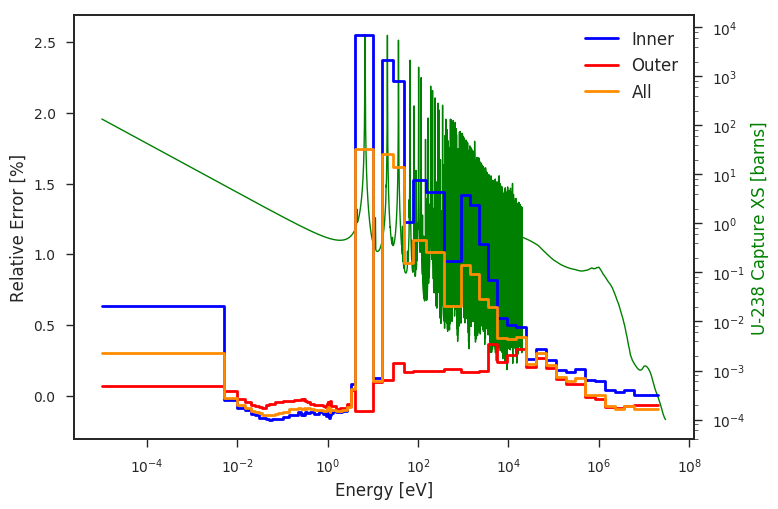
\includegraphics[width=\linewidth]{figures/rel-err-inner-outer}
\caption{The energy-dependent relative error of the OpenMOC scalar flux with respect to the reference OpenMC flux for the innermost, outermost and all FSRs.}
\label{fig:rel-err-energy}
\end{figure}

\begin{figure}[h!]
\centering
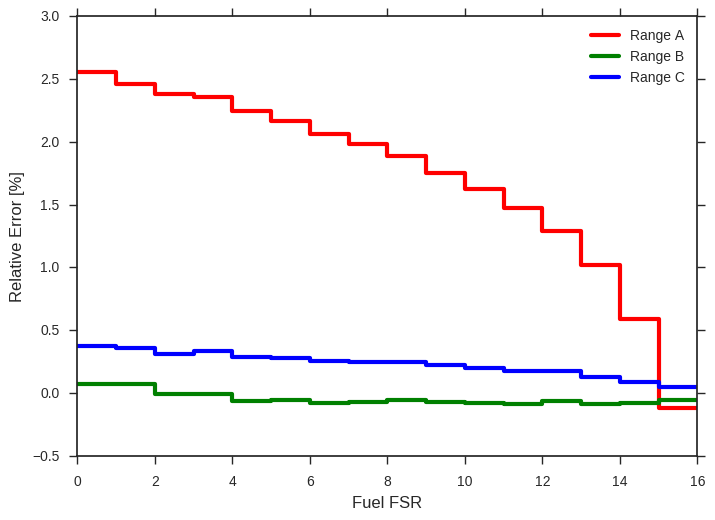
\includegraphics[width=\linewidth]{figures/rel-err-fuel-fsrs}
\caption{The spatially-varying relative error of the OpenMOC scalar flux with respect to the reference OpenMC flux in energy Ranges A, B, and C.}
\label{fig:rel-err-space}
\end{figure}

\begin{figure}[h!]
\centering
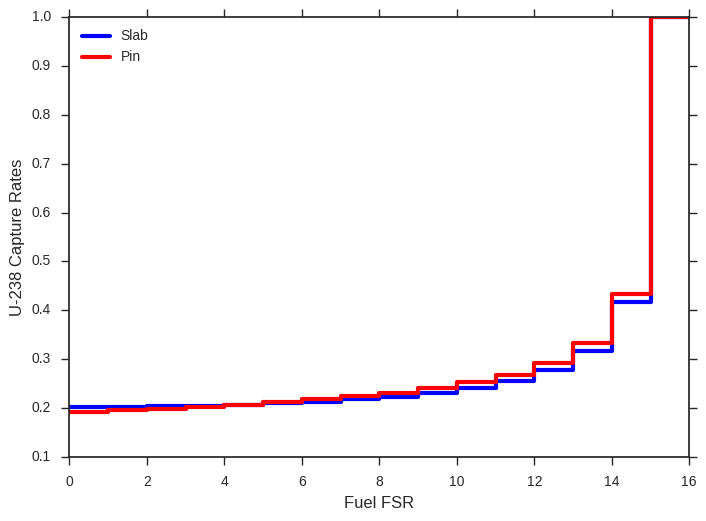
\includegraphics[width=\linewidth]{figures/u238-capt-rates-fuel-fsrs}
\caption{The normalized spatially-varying U-238 capture rates tallied by OpenMC in Range A.}
\label{fig:u238-capture-space}
\end{figure}
